\section{Python}\label{python}
This section will shortly give an overview of the Python programming language version 3.5.1.
This section is based on \citet{python_docs}.

\subsection{About Python}
The Python programming language is a dynamic, interpreted programming language created by Guido van Rossum in the early 1990s.
Python supports multiple programming paradigms, including object oriented and functional programming.
The design philosophy of python values code readability and expressivity.

\subsection{Parsing Python}
A Python program uses newlines as delimiters between statements.\footnote{A line can be joined with the next line if it has a ``\texttt{\textbackslash}'' at the end of the line.}
But if an expression is stretched over several lines for instance in parentheses it is still one line but several physical lines.
A comment starts with a ``\texttt{\#}'' symbol.
Indentation is used for grouping statements for instance a body of a function.
A file is a module which contains definitions and statements and ends with the suffix \texttt{.py}.
A program can contain several modules.

\subsection{Objects}
All data in Python is represented as objects.
An object consists of an identity, a type and a value.
The identity of an object never changes and is represented as an integer.
The type of an object defines how the object can be used and which operations are supported by the object.
The value of an object can for some objects change.
Objects whose value can be changed are called mutable, while objects whose value can not be changed are immutable.

Definition of objects happen in class definitions.
Classes have methods and attributes attached to it.
In \cref{class_definition} a class is defined.
The \texttt{\_\_init\_\_()} method is an initializer function which is called when a new instance is created of that class.
The \texttt{self} keyword references instance variables and instance methods.
This example defines the \texttt{MyClass} class which has one instance method \texttt{print\_i} and one instance variable \texttt{i}.
An instance of this class is created with the value five passed to the \texttt{i} variable through the initializer.
The \texttt{print\_i()} instance method is then called, which will print the value of \texttt{i}.

\begin{lstlisting}[style=python, caption={Class definition}, label=class_definition]
def MyClass(object):
    def __init__(self, i):
        self.i = i

    def print_i(self):
        print('Now i is:' +  i)

mc = MyClass(5)
mc.print_i()        
\end{lstlisting}

\subsection{Collections}
Python contains a number of built in collection classes used to store items in a structured way.
The following will shortly describe the most common collections and their uses, based on \citet{python_datastructures} where additional information can also be found.
The mentioned operations will be exemplified in \cref{collections}.


\paragraph{Lists} A list is a mutable sequence of items.
A list can be appended and extended items, and membership testing can be performed with the \texttt{in} keyword.
A list is iterable and can be indexed to retrieve individual items.
Lists are created with square brackets or the \texttt{list()} function.

\paragraph{Tuples} A tuple is similar to a list, but is an immutable sequence of a number of values.
A tuple is created with round brackets or the \texttt{tuple()} function.

\paragraph{Sets} A set is an implementation of the mathematical set.
It is an unordered collection that contains no duplicates.
A set is created with curly brackets or the \texttt{set()} function.

\paragraph{Dictionaries} A dictionary is an associative map, mapping a key to an item.
The key can be any immutable type which can then be extracted as when indexing a list.
Dictionaries are constructed with curly brackets contained key-value pairs or with the \texttt{dict()} function.

\begin{lstlisting}[style=python, caption={Usage of Python collections}, label=collections]
l = [1, 2, 3, 4] # a list of 4 elements - 1, 2, 3, 4
l.append(9) # append to the list -> 1, 2, 3, 4, 9

s = (5, 6, 7, 8, 8, 8, 8) # a set of 4 elements - 5, 6, 7, 8
l.extend(s) # extend the list with the set
            # -> 1, 2, 3, 4, 10, 5, 6, 7, 8

l.sort() # sort the list
l # the sorted list -> 1, 2, 3, 4, 5, 6, 7, 8, 9

t1 = (1,2) # a tuple -> (1,2)
t1[1] # retrieve the element at index 1 -> 2

t2 = (3,4) # another tuple -> (3,4)

d = dict([t1,t2]} # creating a dictionary from a list of tuples
                  # -> {1 : 2, 3 : 4}
d[1] # retrive item at key 1 - 2
  
d[1] in l # membership testing. Is 2 in l? -> True
    
for element in l: # iterating over the list
    print(element) 
    
\end{lstlisting}

\subsection{Control Structures}\label{python:control_structures}
The python programming language has three control structures, \texttt{if}, \texttt{while} and \texttt{for}.
In the following they are presented with simple code examples and a figure showing the possible information flow through the control structure.

\paragraph{If}
The \texttt{if} control structure has several variants:
\begin{enumerate}
\item A simple \texttt{if} statement
\item An \texttt{if-else} statement
\item An \texttt{if-elif-else} statement where the \texttt{elif} statement can be repeated
\end{enumerate}

\Cref{python:if:simple} shows a simple \texttt{if} control structure containing only one \texttt{if} statement.
The code, \cref{python:if:simple:code}, is an \texttt{if} statement with a condition, \texttt{True}.
If the condition holds the body is executed and if not, the program moves on to the next piece of code.
This flow is depicted on \cref{python:if:simple:flow}.

\begin{figure}[H]
  \centering
  \begin{subfigure}[b]{0.4\textwidth}
    \begin{lstlisting}[style=python]
if True:
    x = 0
    \end{lstlisting}
    \caption{Code example}
    \label{python:if:simple:code}
  \end{subfigure}
  ~ %add desired spacing between images, e. g. ~, \quad, \qquad, \hfill etc. 
  %(or a blank line to force the subfigure onto a new line)
  \begin{subfigure}[b]{0.4\textwidth}
    \centering
    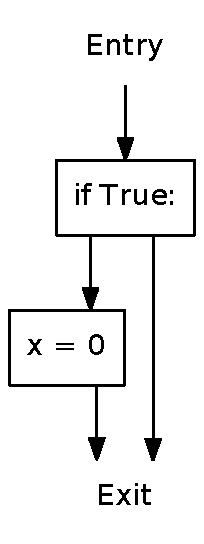
\includegraphics[scale=.4]{./figures/if.pdf}
    \caption{Possible flows}
    \label{python:if:simple:flow}
  \end{subfigure}
  \caption{A simple \texttt{if} control structure containing one \texttt{if} statement}
  \label{python:if:simple}
\end{figure}

The two other variants of the \texttt{if} control structure utilise the \texttt{else} clause to define what should be executed if the condition is \texttt{False}.
This \texttt{else} clause can be a statement body, or a nested \texttt{if} which is denoted as an \texttt{elif}.
An example of this can be seen on \cref{python:if:elif}.
The outmost \texttt{if} has a nested \texttt{elif} statement which then contains a body executed when the \texttt{elif} condition evaluates to \texttt{True} and an \texttt{else} executed when it evaluates to \texttt{False}.

\textbf{Note} that the \textit{else} clause is not represented as a independent node, the false branch is represented in the same way as the true branch in a ``if-else'' structure.

\begin{figure}[H]
  \centering
  \begin{subfigure}[b]{0.4\textwidth}
    \begin{lstlisting}[style=python]
if True:
    x = 0
elif False:
    y = 0
else:
    z = 0
    \end{lstlisting}
    \caption{Code example}
    \label{python:if:elif:code}
  \end{subfigure}
  ~ %add desired spacing between images, e. g. ~, \quad, \qquad, \hfill etc. 
  %(or a blank line to force the subfigure onto a new line)
  \begin{subfigure}[b]{0.4\textwidth}
    \centering
    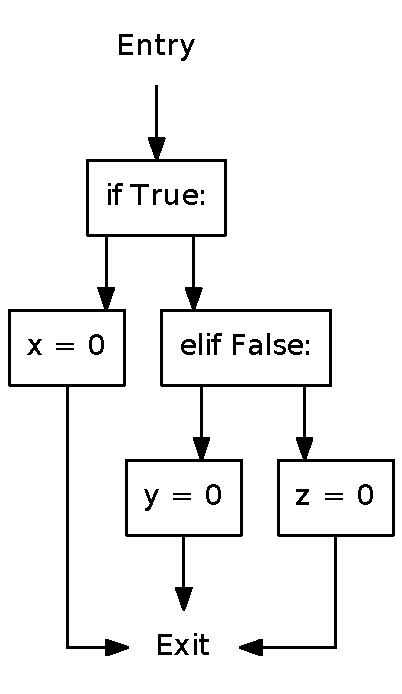
\includegraphics[scale=.4]{./figures/if_else_elif.pdf}
    \caption{Possible flows}
    \label{python:if:elif:flow}
  \end{subfigure}
  \caption{An \texttt{if} control structure containing an \texttt{if}, an \texttt{elif}, and an \texttt{else} statement}
  \label{python:if:elif}
\end{figure}



\paragraph{While}
The \texttt{while} control structure has a condition which evaluates to true or false.
If the condition is true the body is executed and the condition is evaluated again, if it still holds the body is executed again.
This process continues until the condition is false.
A \texttt{while} control structure can also have an \texttt{else} clause.
The body of the \texttt{else} clause is executed when the condition of the \texttt{while} statement is false.

An example is displayed in \cref{python:while:else} which contains a  \texttt{while} control structure with the condition \texttt{x > 100} and an \texttt{else} clause.
The possible flows can be seen on \cref{python:while:else:flow}, where the \texttt{else} clause is executed when the condition resolves to \texttt{False}.

\begin{figure}[H]
  \centering
  \begin{subfigure}[b]{0.4\textwidth}
    \begin{lstlisting}[style=python]
while x < 100:
    x += 1
    x += 2
else:
    x += 3
    x += 4
    \end{lstlisting}
    \caption{Code example}\label{python:while:else:code}
  \end{subfigure}
  ~ %add desired spacing between images, e. g. ~, \quad, \qquad, \hfill etc. 
  %(or a blank line to force the subfigure onto a new line)
  \begin{subfigure}[b]{0.4\textwidth}
    \centering
    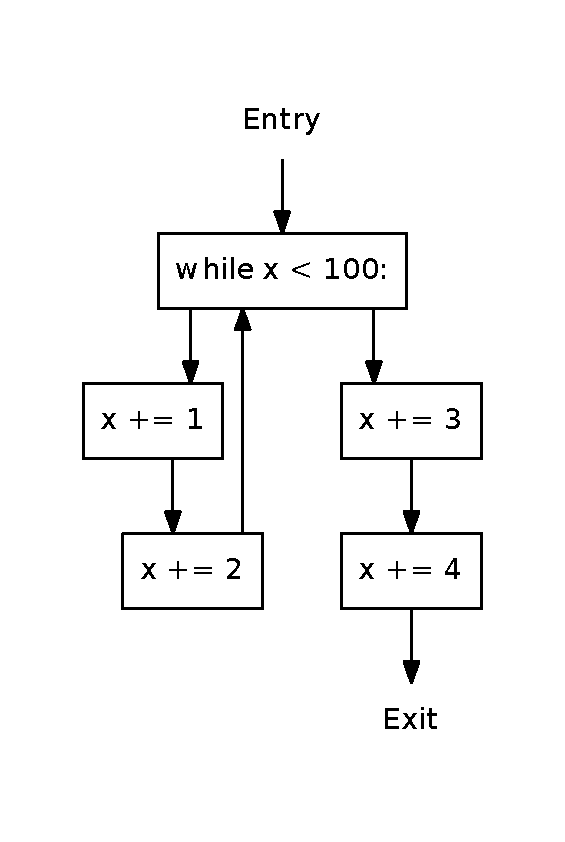
\includegraphics[scale=.4]{./figures/while_else.pdf}
    \caption{Possible flows}
    \label{python:while:else:flow}
  \end{subfigure}
  \caption{A \texttt{while} control structure}
  \label{python:while:else}
\end{figure}


\paragraph{For}
The \texttt{for} control structure is used for iterating over an object that is iterable.
This could for instance be a list or a tuple.
This control structure has an optional \texttt{else} statement, which body is executed when there is nothing to iterate or the \texttt{for} statement is done iterating.
To illustrate the \texttt{for} control structure we provide two examples.
The first example, on \cref{python:for}, shows the most common usage of the \texttt{for} control structure.
Here we iterate over a range, which is a built in function that returns a range of numbers, in this case 0, 1 and 2.

\begin{figure}[H]
  \centering
  \begin{subfigure}[b]{0.4\textwidth}
    \begin{lstlisting}[style=python]
for x in range(3):
    print(x)
    y += 1
x = 3
    \end{lstlisting}
    \caption{Code example}\label{python:for:code}
  \end{subfigure}
  ~ %add desired spacing between images, e. g. ~, \quad, \qquad, \hfill etc. 
  %(or a blank line to force the subfigure onto a new line)
  \begin{subfigure}[b]{0.4\textwidth}
    \centering
    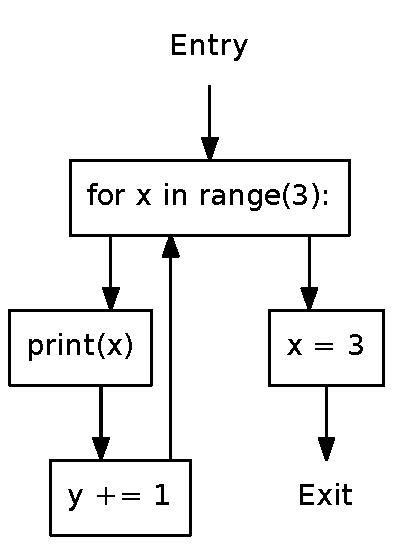
\includegraphics[scale=.5]{./figures/for.pdf}
    \caption{Possible flows}
    \label{python:for:flow}
  \end{subfigure}
  \caption{A \texttt{for} control structure}
  \label{python:for}
\end{figure}
